\chapter{Background and Related Work}\label{ch:2}
\lipsum[1-3]

The remaining chapters are organised as described in \cref{ch:3}; \cref{app:A} contains derivations \citep{ch2-1,ch2-2}.

\section{Overview and Motivation}\label{sec:c2s1}
\kant[3-11]

This section builds on the material in \cref{ch:2}, \cref{ch:3} and the prior work of \citet{ch2-14}; see also \citep{ch2-1,ch2-2}.

\begin{align}\label{eq:c2s1-a}
  \mathbf{x}_{k+1} &= \mathbf{A}\mathbf{x}_k + \mathbf{B}\mathbf{u}_k + \mathbf{w}_k, & \mathbf{w}_k&\sim\mathcal{N}(0,\mathbf{Q}),\\
  \mathbf{y}_k &= \mathbf{C}\mathbf{x}_k + \mathbf{v}_k, & \mathbf{v}_k&\sim\mathcal{N}(0,\mathbf{R}).\label{eq:c2s1-b}
\end{align}

Equations~\eqref{eq:c2s1-a} and~\eqref{eq:c2s1-b} are used throughout the remainder of this section.

\kant[9-11]

\subsection{Quantitative behaviour}\label{sec:c2s1-q}
Results are collected in \cref{tab:c2s1} and visualised in \cref{fig:c2s1-f1}. Similar trends were reported in~\citep{ch2-12,ch2-6}.

\begin{table}[htbp]
\centering
\caption{Summary of measured quantities for experiment set \texttt{c2s1}.}\label{tab:c2s1}
\begin{tabular}{lrrr}
\toprule
Method & Score & Latency & Error \\
\midrule
Alpha & \num{56.7} & \SI{9.27}{\milli\second} & \num{5.017e-1} \\
Beta & \num{90.1} & \SI{0.37}{\milli\second} & \num{4.719e-3} \\
Gamma & \num{93.9} & \SI{3.82}{\milli\second} & \num{8.134e-5} \\
Delta & \num{17.8} & \SI{5.59}{\milli\second} & \num{2.889e-1} \\
Epsilon & \num{19.0} & \SI{3.29}{\milli\second} & \num{2.094e-5} \\
\bottomrule
\end{tabular}
\end{table}

\begin{figure}[htbp]
\centering
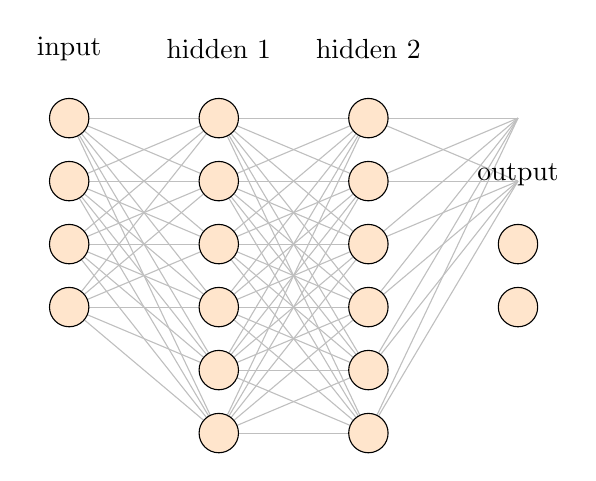
\begin{tikzpicture}[x=1.9cm,y=0.8cm,neuron/.style={circle,draw,fill=orange!20,minimum size=5mm,inner sep=0}]
\foreach \i in {1,...,4}{\foreach \j in {1,...,6}{\draw[gray!50](0,-\i)--(1,-\j);}}
\foreach \i in {1,...,6}{\foreach \j in {1,...,6}{\draw[gray!50](1,-\i)--(2,-\j);}}
\foreach \i in {1,...,6}{\foreach \j in {1,...,2}{\draw[gray!50](2,-\i)--(3,-\j);}}
\foreach \i in {1,...,4}\node[neuron](i\i)at(0,-\i){};
\foreach \i in {1,...,6}\node[neuron](h\i)at(1,-\i){};
\foreach \i in {1,...,6}\node[neuron](g\i)at(2,-\i){};
\foreach \i in {1,...,2}\node[neuron](o\i)at(3,-\i-2){};
\node at(0,0.1){input};\node at(1,0.1){hidden 1};\node at(2,0.1){hidden 2};\node at(3,-1.9){output};
\end{tikzpicture}
\caption{Generated figure for \texttt{c2s1-f1} (parameters $a=4$, $b=4$).}\label{fig:c2s1-f1}
\end{figure}

\kant[6-12]

\subsection{Implementation notes}\label{sec:c2s1-i}
The core routine is shown in \cref{lst:c2s1}; its complexity is $\mathcal{O}(N\log N)$ per iteration~\cite{ch2-3}.

\begin{lstlisting}[language=c,caption={Reference implementation for c2s1.},label={lst:c2s1}]
#include <stdio.h>

/* Compute a dot product of two vectors. */
double dot(const double *a, const double *b, int n) {
    double s = 0.0;
    for (int i = 0; i < n; ++i)
        s += a[i] * b[i];
    return s;
}
\end{lstlisting}

\lipsum[91-91]
\begin{theorem}\label{thm:c2s1}
Let $A\in\mathbb{R}^{n\times n}$ be symmetric positive definite with condition number $\kappa$. Then the iteration converges and
$\lVert e_k\rVert_A \le 2\bigl(\tfrac{\sqrt\kappa-1}{\sqrt\kappa+1}\bigr)^k\lVert e_0\rVert_A$.
\end{theorem}
\begin{enumerate}[label=(\roman*)]
\item the bound in \cref{thm:c2s1} is sharp for some initial errors;
\item the constant $2$ cannot be improved in general;
\item preconditioning reduces the effective $\kappa$.
\end{enumerate}

\begin{figure}[htbp]
\centering
\includegraphics[width=0.45\linewidth]{checker.png}
\caption{Raster/vector asset \texttt{checker.png} included from the figures directory.}\label{fig:c2s1-i0}
\end{figure}

\lipsum[115-115]

\section{Mathematical Framework}\label{sec:c2s2}
\lipsum[128-128]

This section builds on the material in \cref{sec:c2s1}, \cref{ch:3} and the prior work of \citet{ch2-13}; see also \citep{ch2-7,ch2-12}.

\begin{equation}\label{eq:c2s2-a}
  I = \int_{0}^{1}\!\!\int_{0}^{1} \frac{\sin(\pi x)\sin(\pi y)}{1+x^2+y^2}\,\mathrm{d}x\,\mathrm{d}y \approx \frac{1}{M}\sum_{m=1}^{M} h(\xi_m),
\end{equation}
with variance decreasing as
\begin{equation}\label{eq:c2s2-b}
  \operatorname{Var}\bigl[\hat I_M\bigr] = \frac{1}{M}\Bigl(\int h^2\,\mathrm{d}\mu - I^2\Bigr) = \mathcal{O}(M^{-1}).
\end{equation}

Equations~\eqref{eq:c2s2-a} and~\eqref{eq:c2s2-b} are used throughout the remainder of this section.

\kant[8-11]

\subsection{Quantitative behaviour}\label{sec:c2s2-q}
Results are collected in \cref{tab:c2s2} and visualised in \cref{fig:c2s2-f1}. Similar trends were reported in~\citep{ch2-8,ch2-9}.

\begin{table}[htbp]
\centering
\caption{Summary of measured quantities for experiment set \texttt{c2s2}.}\label{tab:c2s2}
\begin{tabular}{lrrr}
\toprule
Method & Score & Latency & Error \\
\midrule
Alpha & \num{36.9} & \SI{5.66}{\milli\second} & \num{8.363e-4} \\
Beta & \num{50.8} & \SI{6.56}{\milli\second} & \num{8.525e-2} \\
Gamma & \num{90.7} & \SI{9.00}{\milli\second} & \num{3.145e-4} \\
Delta & \num{32.6} & \SI{3.07}{\milli\second} & \num{7.394e-5} \\
Epsilon & \num{58.5} & \SI{5.17}{\milli\second} & \num{6.211e-5} \\
\bottomrule
\end{tabular}
\end{table}

\begin{figure}[htbp]
\centering
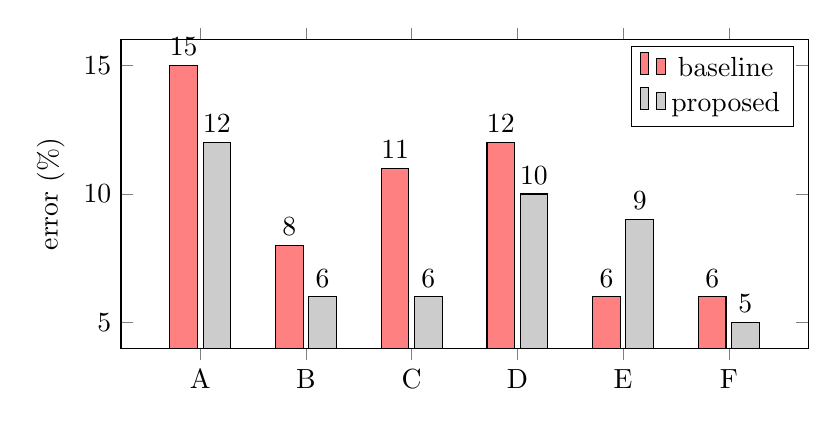
\begin{tikzpicture}\begin{axis}[ybar,width=0.85\linewidth,height=5.5cm,symbolic x coords={A,B,C,D,E,F},xtick=data,ylabel={error (\%)},enlarge x limits=0.15,bar width=10pt,nodes near coords]
\addplot[fill=red!50] coordinates {(A,15) (B,8) (C,11) (D,12) (E,6) (F,6)};
\addplot[fill=gray!40] coordinates {(A,12) (B,6) (C,6) (D,10) (E,9) (F,5)};
\legend{baseline,proposed}
\end{axis}\end{tikzpicture}
\caption{Generated figure for \texttt{c2s2-f1} (parameters $a=5$, $b=6$).}\label{fig:c2s2-f1}
\end{figure}

\lipsum[126-127]

\subsection{Implementation notes}\label{sec:c2s2-i}
The core routine is shown in \cref{lst:c2s2}; its complexity is $\mathcal{O}(N\log N)$ per iteration~\cite{ch2-4}.

\begin{lstlisting}[language=c,caption={Reference implementation for c2s2.},label={lst:c2s2}]
#include <stdio.h>

/* Compute a dot product of two vectors. */
double dot(const double *a, const double *b, int n) {
    double s = 0.0;
    for (int i = 0; i < n; ++i)
        s += a[i] * b[i];
    return s;
}
\end{lstlisting}

\kant[6-12]
\begin{theorem}\label{thm:c2s2}
Let $A\in\mathbb{R}^{n\times n}$ be symmetric positive definite with condition number $\kappa$. Then the iteration converges and
$\lVert e_k\rVert_A \le 2\bigl(\tfrac{\sqrt\kappa-1}{\sqrt\kappa+1}\bigr)^k\lVert e_0\rVert_A$.
\end{theorem}
\begin{enumerate}[label=(\roman*)]
\item the bound in \cref{thm:c2s2} is sharp for some initial errors;
\item the constant $2$ cannot be improved in general;
\item preconditioning reduces the effective $\kappa$.
\end{enumerate}

\begin{figure}[htbp]
\centering
\includegraphics[width=0.45\linewidth]{waves.png}
\caption{Raster/vector asset \texttt{waves.png} included from the figures directory.}\label{fig:c2s2-i0}
\end{figure}

\kant[4-12]

\section{Analysis and Validation}\label{sec:c2s3}
\kant[3-11]

This section builds on the material in \cref{sec:c2s2}, \cref{ch:3} and the prior work of \citet{ch2-2}; see also \citep{ch2-1,ch2-10}.

\begin{equation}\label{eq:c2s3-a}
  \hat{\theta} = \arg\min_{\theta\in\Theta}\; \frac{1}{n}\sum_{i=1}^{n}\ell\bigl(y_i, g_\theta(x_i)\bigr) + \lambda\lVert\theta\rVert_2^2 .
\end{equation}
Under standard regularity conditions the estimator is consistent, and its error satisfies
\begin{equation}\label{eq:c2s3-b}
  \mathbb{E}\lVert\hat\theta-\theta^\star\rVert^2 \le \frac{C\,\sigma^2 d}{n} + \lambda^2\lVert\theta^\star\rVert^2 .
\end{equation}

Equations~\eqref{eq:c2s3-a} and~\eqref{eq:c2s3-b} are used throughout the remainder of this section.

\kant[1-11]

\subsection{Quantitative behaviour}\label{sec:c2s3-q}
Results are collected in \cref{tab:c2s3} and visualised in \cref{fig:c2s3-f1}. Similar trends were reported in~\citep{ch2-11,ch2-13}.

\begin{table}[htbp]
\centering
\caption{Summary of measured quantities for experiment set \texttt{c2s3}.}\label{tab:c2s3}
\begin{tabular}{lrrr}
\toprule
Method & Score & Latency & Error \\
\midrule
Alpha & \num{92.9} & \SI{7.13}{\milli\second} & \num{1.255e-3} \\
Beta & \num{37.8} & \SI{1.78}{\milli\second} & \num{6.382e-1} \\
Gamma & \num{12.7} & \SI{9.45}{\milli\second} & \num{1.203e-1} \\
Delta & \num{39.2} & \SI{2.61}{\milli\second} & \num{7.507e-2} \\
Epsilon & \num{76.2} & \SI{1.90}{\milli\second} & \num{6.532e-4} \\
\bottomrule
\end{tabular}
\end{table}

\begin{figure}[htbp]
\centering
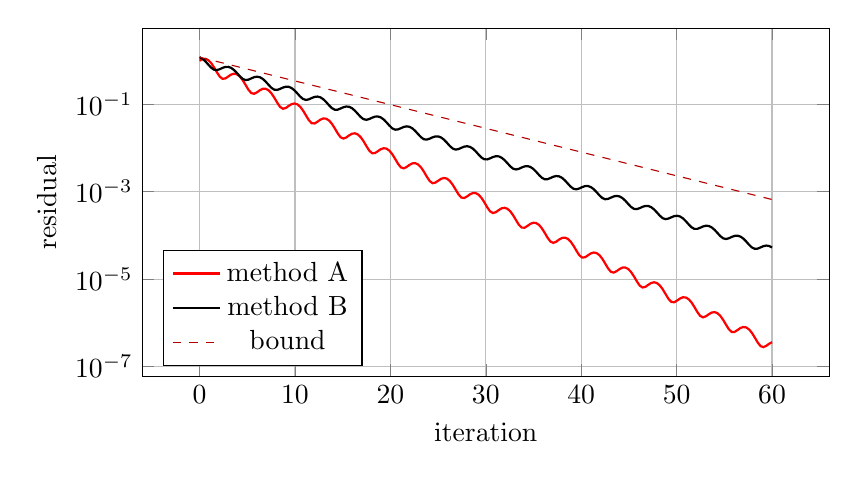
\begin{tikzpicture}\begin{semilogyaxis}[width=0.85\linewidth,height=6cm,xlabel={iteration},ylabel={residual},domain=0:60,grid=major,legend pos=south west]
\addplot[red,thick,samples=200]{exp(-x/4)*(1+0.3*sin(deg(x*2)))};
\addplot[black,thick,samples=200]{exp(-x/6)*(1+0.2*cos(deg(x*2)))};
\addplot[red!70!black,dashed,samples=200]{1.2*exp(-x/8)};
\legend{method A,method B,bound}
\end{semilogyaxis}\end{tikzpicture}
\caption{Generated figure for \texttt{c2s3-f1} (parameters $a=2$, $b=4$).}\label{fig:c2s3-f1}
\end{figure}

\lipsum[10-11]

\subsection{Implementation notes}\label{sec:c2s3-i}
The core routine is shown in \cref{lst:c2s3}; its complexity is $\mathcal{O}(N\log N)$ per iteration~\cite{ch2-5}.

\begin{lstlisting}[language=python,caption={Reference implementation for c2s3.},label={lst:c2s3}]
def conjugate_gradient(A, b, tol=1e-8, maxit=500):
    x = b * 0
    r = b - A @ x
    p = r.copy()
    for k in range(maxit):
        Ap = A @ p
        alpha = (r @ r) / (p @ Ap)
        x += alpha * p
        r_new = r - alpha * Ap
        if (r_new @ r_new) ** 0.5 < tol:
            break
        p = r_new + ((r_new @ r_new) / (r @ r)) * p
        r = r_new
    return x
\end{lstlisting}

\lipsum[29-29]
\begin{theorem}\label{thm:c2s3}
Let $A\in\mathbb{R}^{n\times n}$ be symmetric positive definite with condition number $\kappa$. Then the iteration converges and
$\lVert e_k\rVert_A \le 2\bigl(\tfrac{\sqrt\kappa-1}{\sqrt\kappa+1}\bigr)^k\lVert e_0\rVert_A$.
\end{theorem}
\begin{enumerate}[label=(\roman*)]
\item the bound in \cref{thm:c2s3} is sharp for some initial errors;
\item the constant $2$ cannot be improved in general;
\item preconditioning reduces the effective $\kappa$.
\end{enumerate}

\lipsum[126-126]

\unitbib{Chapters/refs-ch2}
